%%%%%%%%%%%%%%%%%%%%%%%%%%%%%%%%%%%%%%%%%%%%%%%%%%%%%%%%%%%%%%%%%%%%%%
%%                     Uncertain Process
%%%%%%%%%%%%%%%%%%%%%%%%%%%%%%%%%%%%%%%%%%%%%%%%%%%%%%%%%%%%%%%%%%%%%%
%\color{blue}
\subsection{Glyph: \glyph{Uncertain process}}\label{sec:uncertain}

Uncertain processes are processes that may not exist. A single \glyph{uncertain process} can represent any number of actual processes.

\begin{glyphDescription}
 \item[SBO]\mbox{}\\ To be determined
 \item[origin]\mbox{}\\ One or several \glyph{consumption} arcs (section \ref{sec:consumption}) or one or several \glyph{production} arcs (section \ref{sec:production}).
 \item[target]\mbox{}\\ One or several \glyph{production} arcs (section \ref{sec:production}).
 \item[node]\mbox{}\\ Uncertain processes are represented as a transition containing a questionmark.
 \end{glyphDescription}

\begin{figure}[H]
  \centering
  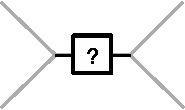
\includegraphics[scale = 0.5]{images/uncertain}
  \caption{The \PD glyph for \glyph{uncertain}.}
  \label{fig:uncertain}
\end{figure}

